\definecolor{tttttt}{rgb}{0.2,0.2,0.2}
%dash pattern=on 5pt off 2pt
%[fill = white, rounded corners = 5pt, inner sep=0.8pt]
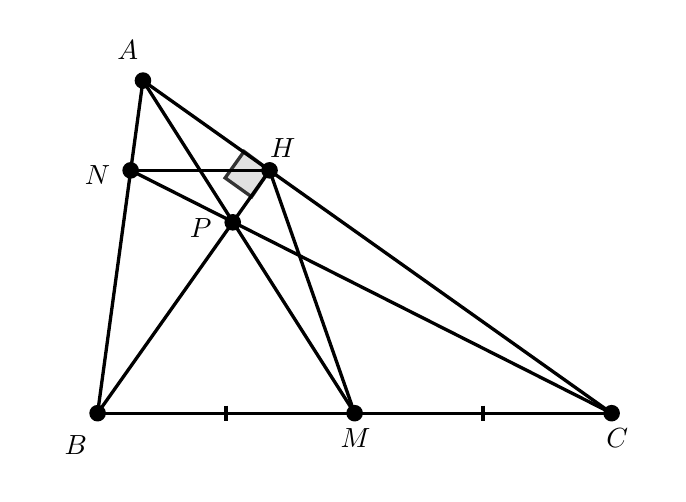
\begin{tikzpicture}[scale = 1.2]
    \clip(-1.96,0.22) rectangle (4.71,4.94);
    \draw[line width=1.2pt,color=tttttt,fill=tttttt,fill opacity=0.15] (0.33,3.63) -- (0.13,3.35) -- (0.41,3.15) -- (0.6,3.43) -- cycle;
    \draw [line width=1.2pt] (-0.74,4.38)-- (-1.22,0.86);
    \draw [line width=1.2pt] (4.22,0.86)-- (-0.74,4.38);
    \draw [line width=1.2pt] (-0.74,4.38)-- (1.5,0.86);
    \draw [line width=1.2pt] (-1.22,0.86)-- (0.6,3.43);
    \draw [line width=1.2pt] (-0.87,3.43)-- (4.22,0.86);
    \draw [line width=1.2pt] (-0.87,3.43)-- (0.6,3.43);
    \draw [line width=1.2pt] (1.5,0.86)-- (0.6,3.43);
    \draw [line width=1.2pt] (-1.22,0.86)-- (1.5,0.86);
    \draw [line width=1.2pt] (0.14,0.94) -- (0.14,0.78);
    \draw [line width=1.2pt] (1.5,0.86)-- (4.22,0.86);
    \draw [line width=1.2pt] (2.86,0.94) -- (2.86,0.78);
    \begin{scriptsize}
        \normalsize
        \fill [color=black] (-0.74,4.38) circle (2.5pt);
        \draw[color=black] (-0.9,4.7) node {$A$};
        \fill [color=black] (-1.22,0.86) circle (2.5pt);
        \draw[color=black] (-1.45,0.52) node {$B$};
        \fill [color=black] (4.22,0.86) circle (2.5pt);
        \draw[color=black] (4.28,0.6) node {$C$};
        \fill [color=black] (1.5,0.86) circle (2.5pt);
        \draw[color=black] (1.51,0.6) node {$M$};
        \fill [color=black] (0.6,3.43) circle (2.5pt);
        \draw[color=black] (0.74,3.67) node {$H$};
        \fill [color=black] (-0.87,3.43) circle (2.5pt);
        \draw[color=black] (-1.22,3.38) node {$N$};
        \fill [color=black] (0.21,2.88) circle (2.5pt);
        \draw[color=black] (-0.13,2.82) node[fill = white, rounded corners = 5pt, inner sep=0.8pt] {$P$};
    \end{scriptsize}
\end{tikzpicture}